\chapter{Simulations} \label{ch:simulation}

\section{Computational Aspects}
Assume that we have $(Z_i, \delta_i)_{i\leq n}$ is a sample in the sense of RCM. Define the target value 
$$\theta^* := \int_{0}^{\tau_H}\int_{0}^{\tau_H} \phi(s,t) F(ds)F(dt)$$
and denote $U_n$ an estimator for $\theta^*$. In the following, we will estimate the above for different kernels $\phi$ under different censoring models $m$ for $F_n^{se}$. For the simulation, one chooses first an appropriate censoring model $m$ in connection with the compatible distribution for $X$ and/or $Y$. The kernel $\phi$ can be chosen separately. Then the Maximum Likelihood estimate for $\hat\theta_n$ is calculated. Afterwards, the Kaplan-Meier and the semiparametric weights are calculated, using the following formulas
$$W_{i,n}^{se} = F_n^{se}(Z_{i:n}) - F_n^{se}(Z_{i-1:n}) = \frac{m(Z_{i:n},\hat\theta_n)}{n-i+1} \prod\limits_{k=1}^{i-1}\left[1-\frac{m(Z_{k:n},\hat\theta_n)}{n-k+1}\right]$$
and 
$$W_{i,n}^{km} = F_n^{km}(Z_{i:n}) - F_n^{km}(Z_{i-1:n}) = \frac{\delta_{[i:n]}}{n-i+1} \prod\limits_{k=1}^{i-1}\left[1-\frac{\delta_{[k:n]}}{n-k+1}\right]$$
respectively. Now the normalized versions of the Kaplan-Meier and the semiparametric U-statistics can be calculated as
$$U_n^{se} = \doublesum\limits_{1\leq i < j \leq n} \phi(Z_{i:n}, Z_{j:n}) W_{i,n}^{se} W_{j,n}^{se}$$
and 
$$U_n^{km} = \doublesum\limits_{1\leq i < j \leq n} \phi(Z_{i:n}, Z_{j:n}) W_{i,n}^{km} W_{j,n}^{km}$$
%\\
\\
As kernel for the following simulation studies, we choose 
$$\phi(x_1,x_2) = \frac{1}{2} (x_1 - x_2)^2\mdot$$
Hence we are estimating the sample variance, as pointed out in example \ref{ex:phi}. The semiparametric and the Kaplan-Meier estimates of $\theta^*$ will be denoted as $\sigma_{n}^{se}$ and $\sigma_{n}^{km}$. Each simulation is repeated $M = 100$ times for different samples of size $n$. Let $((Z_i, \delta_i)_{i\leq n})_{j\leq M}$ be the collection of $M$ independent RCM samples generated and let $\sigma_n \in \{\sigma_n^{se}, \sigma_n^{km}\}$. We will write $\sigma_{n,j}$ estimate of $\theta^*$ based on sample $((Z_i, \delta_i)_{i\leq n})_j$ for $j=1,\dots,M$. The Bias of $\sigma_n$ will be calculated by the following formula
$$Bias(\sigma_n) = \frac{1}{M}\sum_{j=1}^{M}(\sigma_{n,j} - \theta^*)\mdot$$
For the Variance of $\sigma_n$ we use
$$Var(\sigma_n) = \frac{1}{M-1}\sum_{j=1}^{M}(\sigma_{n,j} - \bar\sigma_M)^2 \quad\text{ with }\quad \bar\sigma_M = \frac{1}{M} \sum_{j=1}^{M} \sigma_{n,j}\mdot$$
The mean squared error (MSE) will be estimated by
$$MSE(\sigma_n) = \frac{1}{M}\sum_{j=1}^{M}(\sigma_{n,j} - \theta^*)^2$$. 
Furthermore we will calculate quantiles of $F_n^{km}$ and $F_n^{se}$, by
$$q_n^{se}(p) = \inf\{t \in \R_+| F_n^{se}(t) \geq p\}$$
and
$$q_n^{se}(p) = \inf\{t \in \R_+| F_n^{se}(t) \geq p\}\mcomma$$
respectively. In order to get information about the underlying estimates $F_n^{se}$ and $F_n^{km}$ of the true \df\ $F$, we will calculate the Bias, variance and MSE for $q_n^{se}(p)$ and $q_n^{km}(p)$ as well. The simulation results will be displayed in two tables. One table contains bias, variance and MSE of $\sigma_n^{se}$ and $\sigma_{n}^{km}$. The other table shows the bias and MSE of $q_n^{se}(p)$ and $q_n^{km}(p)$ for $p\in\{0.25, 0.5, 0.75\}$. The results are also illustrated by a figure at the end of each section. The left image shows the \textbf{squared} Bias, variance and MSE for $\sigma_n^{se}$ and $\sigma_n^{km}$. The right image displays the MSE of $q_n^{se}(p)$ and $q_n^{km}(p)$ for $p\in\{0.25, 0.5, 0.75\}$.
%
%
%
\section{Simulation 1} \label{sec:sim_expexp}
Suppose $X \sim Exp(\alpha)$ and $Y\sim Exp(\beta)$. Then we have
$$m(z,\theta) = \frac{\alpha}{\alpha + \beta}\mdot$$
Note that $m$ is constant in this case. Hence we are in the situation of proportional hazards model, as described in \ref{ex:intro_phm}.\\
\\
For this simulation, we chose $\alpha = 2$ and $\beta = 1$. The target value was here
$$Var(X) = \frac{1}{\alpha^2}=\frac{1}{4}\mdot$$

\clearpage
\begin{figure}[h!]
	\begin{center}
		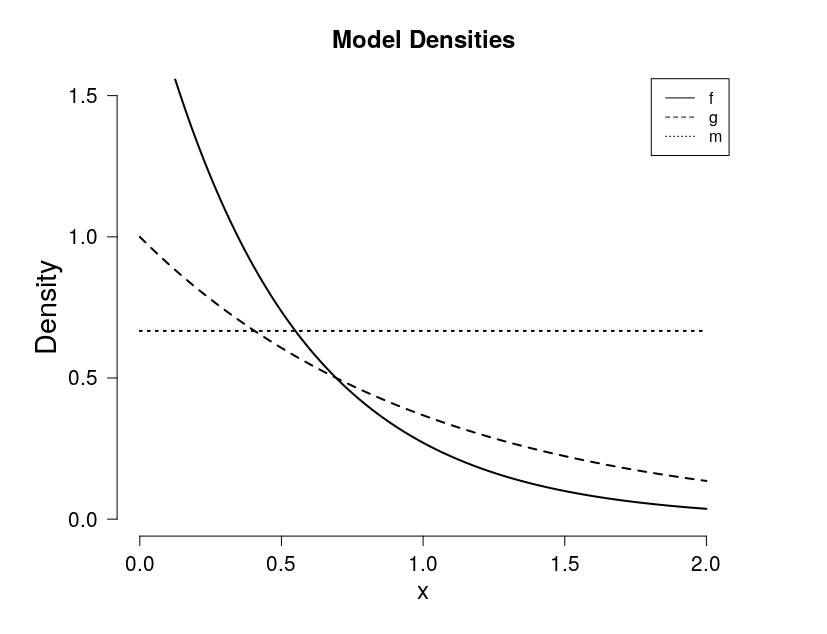
\includegraphics[width=0.8\textwidth]{./figures/exp_exp_dens}
	\end{center}
	\caption{Probability density functions $f$, $g$ and censoring model $m$ for Simulation 1.}
	\label{fig:dens_expexp}
\end{figure}
Figure \ref{fig:dens_expexp} indicates that larger values will be censored rather than smaller values. 
%$$f(z) = \alpha\beta (\alpha z)^{\beta-1}\exp\left(-(\alpha z)^{\beta}\right)$$
%$$m(z,\theta) = \frac{1}{1+\exp(-\theta z)} \textrm{ with } \theta = \left(\frac{\alpha_2^{\beta_2}\beta_2}{\alpha_1^{\beta_1}\beta_1}, \beta_2 - \beta_1\right)$$
%Then the pdf of $Y$ is given by 
%$$g(z) = 2\alpha^2 z \exp\left(-\theta z\right) \exp\left(\frac{-2\alpha^2(1-(\theta z + 1)\exp(-\theta z))}{\theta^2}\right)\mdot$$
Table \ref{tab:res_expexp1} and table \ref{tab:res_expexp2} show the results of the simulation. A graphical display of the results is depicted in figure \ref{fig:mse_expexp}.
\begin{table}[h!]
	\begin{center}
		%run(n = c(500,1000,5000), theta1 = c(2,1), theta2 = c(1,1))
		\begin{tabular}{| l || c | c | c |}
		\hline
		&       $n=100$   &    $n=500$    &    $n=1000$\\
		\hline
		\hline
%		$Var$ & 0.25 & 0.25 & 0.25\\
%		$U_n^{se}$ & 0.178959 & 0.214204 & 0.228216\\
%		$U_n^km$ & 0.17329 & 0.205476 & 0.226042\\
		$Bias(\sigma_n^{se})$ & -0.071041 & -0.035796 & -0.021784\\
		$Bias(\sigma_n^{km})$ & -0.07671 & -0.044524 & -0.023958\\
		\hline
		$Var(\sigma_n^{se})$ & 0.003708 & 0.00132 & 0.000911\\
		$Var(\sigma_n^{km})$ & 0.009248 & 0.002407 & 0.0019\\
		\hline
		$MSE(\sigma_n^{se})$ & 0.008755 & 0.002601 & 0.001385\\
		$MSE(\sigma_n^{km})$  & 0.015133 & 0.004389 & 0.002474\\
		\hline
		\hline
		$\bar c$  & 0.3247 & 0.33262 & 0.33503\\
		\hline
		\end{tabular}
	\end{center}
	\caption{Results for the variance estimators of Simulation 1.}
	\label{tab:res_expexp1}
\end{table}
%
As we can see, bias, variance and MSE are decreasing to zero for both estimators. The semiparametric estimator is performing clearly better under this setup. Figure \ref{fig:mse_expexp} indicates that the gain in efficiency is greater for smaller sample sizes. Moreover we can see that the gain in efficiency for $\sigma_{n}^{se}$ is more related to the bias, than to the variance. 
\begin{table}[h!]
	\begin{center}
		%run(n = c(500,1000,5000), theta1 = c(2,1), theta2 = c(1,1))
		\begin{tabular}{| l || c | c | c |}
			\hline
			&       $n=100$   &    $n=500$    &    $n=1000$\\
			\hline
			\hline
			$Bias(q^{se}_n(0.25)) $  & -0.009688 & -0.002208 & -0.001151\\
			$Bias(q^{km}_n(0.25)) $  & -0.006024 & -0.001416 & 0.000264\\
			\hline
			$Bias(q^{se}_n(0.5)) $  & -0.014168 & -0.002367 & 0.000564\\
			$Bias(q^{km}_n(0.5))$  & -0.012675 & -0.000372 & 0.002214\\
			\hline
			$Bias(q^{se}_n(0.75))$  & -0.028701 & -0.004343 & 0.004808\\
			$Bias(q^{km}_n(0.75))$  & -0.044761 & -0.007439 & 0.004497\\
			\hline
			\hline
			$MSE(q^{se}_n(0.25))$  & 0.000868 & 0.000144 & 0.00005\\
			$MSE(q^{km}_n(0.25))$  & 0.000809 & 0.000182 & 0.000064\\
			\hline
			$MSE(q^{se}_n(0.5))$  & 0.002608 & 0.000424 & 0.000204\\
			$MSE(q^{km}_n(0.5))$  & 0.002806 & 0.000469 & 0.000258\\
			\hline
			$MSE(q^{se}_n(0.75))$  & 0.009388 & 0.002047 & 0.000695\\
			$MSE(q^{km}_n(0.75))$  & 0.010156 & 0.0021 & 0.000823\\
			\hline
		\end{tabular}
	\end{center}
	\caption{Results for estimated quantiles of Simulation 1.}
	\label{tab:res_expexp2}
\end{table}
\\
The Quantiles are estimated quite well under this setup. The MSE of both $q_{n}^{se}$ and $q_{n}^{km}$ are decreasing. Here $q_{n}^{se}$ is performing slightly better.
\begin{figure}[h!]
	\begin{center}
		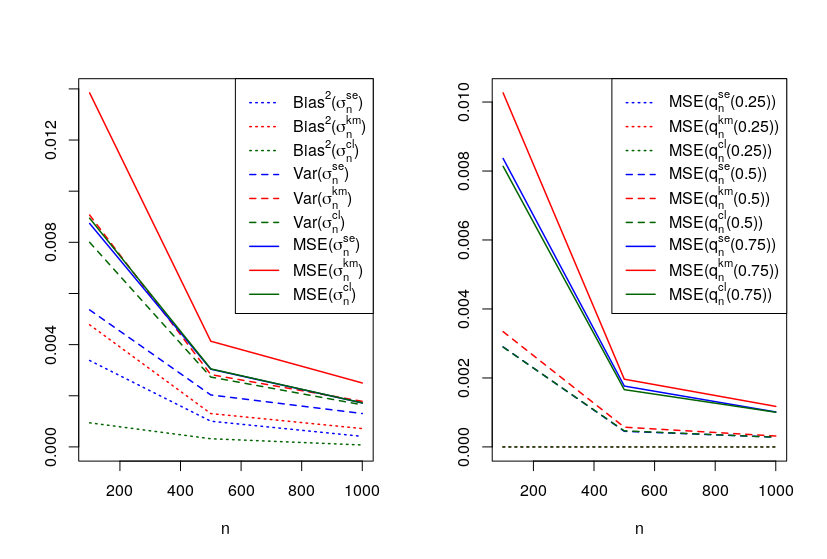
\includegraphics[width=0.9\textwidth]{./figures/expexp_mse2}
	\end{center}
	\caption{Results for Simulation 1. left: bias, variance and MSE for $\sigma_n^{se}$ and $\sigma_n^{km}$. right: MSE for $q_n^{se}$ and $q_n^{km}$.}
	\label{fig:mse_expexp}
\end{figure}
\clearpage
%
%
%
\section{Simulation 2} \label{sec:sim_weiwei}
Let $X \sim Weibull(\alpha_1, \beta_1)$ and  $X \sim Weibull(\alpha_2, \beta_2)$.
%$$f(z) = \alpha_1\beta_1 (\alpha_1 z)^{\beta_1-1}\exp\left(-(\alpha_1 z)^{\beta_1}\right)$$
%$$g(z) = \alpha_2\beta_2 (\alpha_2 z)^{\beta_2-1}\exp\left(-(\alpha_2 z)^{\beta_2}\right)$$
Then we obtain for the censoring model 
$$m(z,\theta) = \frac{1}{1+\theta_1 z^{\theta_2}} \textrm{ with } \theta = \left(\frac{\alpha_2^{\beta_2}\beta_2}{\alpha_1^{\beta_1}\beta_1}, \beta_2 - \beta_1\right)$$
%
For the simulation below we chose $\alpha_1 = 2$, $\alpha_2 = 1$, $\beta_1 = 1.2$ and $\beta_2 = 1$. The target value was here
$$Var(X) = 0.192843234\mdot$$
Figure \ref{fig:dens_wei_wei} shows the pdf's $f$, $g$ and the censoring model $m$ for this setup.\\
\begin{figure}[h!]
	\begin{center}
		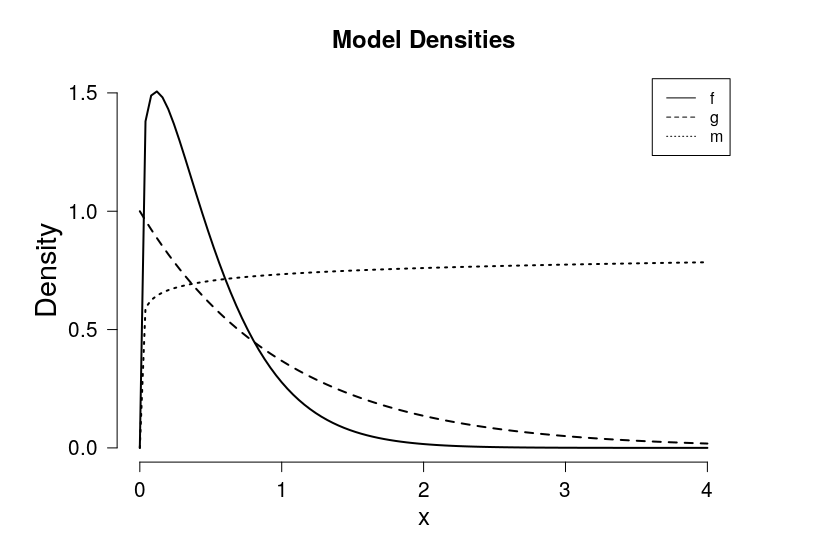
\includegraphics[width=0.8\textwidth]{./figures/wei_wei_dens2}
	\end{center}
	\caption{Probability density functions $f$, $g$ and censoring model $m$ for Simulation 1.}
	\label{fig:dens_wei_wei}
\end{figure}\\
The figure indicates that larger values are censored rather than smaller ones under this setup. Tables \ref{tab:res_weiwei1} and \ref{tab:res_weiwei2} show the results of the simulation. Figure \ref{fig:mse_weiwei} illustrates the results.\\
\clearpage
%
\begin{table}[h!]
	\begin{center}
		%run(n = c(500,1000,5000), theta1 = c(2,1.2), theta2 = c(1,1))
		\begin{tabular}{| l || c | c | c |}
			\hline
			&       $n=100$   &    $n=500$    &    $n=1000$\\
			\hline
			\hline
%			$Var$ & 0.154936 & 0.154936 & 0.154936\\
%			$U_n^{se}$ & 0.13533 & 0.154696 & 0.158717\\
%			$U_n^km$ & 0.134849 & 0.143497 & 0.143514\\
			$Bias(\sigma_n^{se})$ & -0.019606 & -0.000239 & 0.003782\\
			$Bias(\sigma_n^{km})$ & -0.020086 & -0.011439 & -0.011422\\
			\hline
			$Var(\sigma_n^{se})$ & 0.001659 & 0.000669 & 0.000298\\
			$Var(\sigma_n^{km})$ & 0.002861 & 0.000794 & 0.000257\\
			\hline
			$MSE(\sigma_n^{se})$ & 0.002044 & 0.000669 & 0.000312\\
			$MSE(\sigma_n^{km})$ & 0.003265 & 0.000925 & 0.000388\\
			\hline
			\hline
			$\bar c$ & 0.3295 & 0.3322 & 0.33462\\
			\hline
		\end{tabular}
	\end{center}
	\caption{Results for simulation 2 with  $\alpha_1 = \alpha_2 = 1$, $\beta_1 = 2$ and $\beta_2 = 2$.}
	\label{tab:res_weiwei1}
\end{table}
%
As we can see, the Bias and MSE are decreasing nicely to zero for both estimators. The semiparametric estimator is clearly performing better than the Kaplan-Meier PLE \wrt\ the MSE. Here again, the gain in difference in bias is much larger than the difference in variance. Figure \ref{fig:mse_weiwei} indicates again, that the gain in efficiency is greater for smaller sample sizes $n$.
\begin{table}[h!]
	\begin{center}
		%run(n = c(500,1000,5000), theta1 = c(2,1.2), theta2 = c(1,1))
		\begin{tabular}{| l || c | c | c |}
			\hline
			&       $n=100$   &    $n=500$    &    $n=1000$\\
			\hline
			\hline
			$Bias(q^{se}_n(0.25)) $ & -0.018255 & -0.011443 & -0.011854\\
			$Bias(q^{km}_n(0.25)) $ & -0.007356 & -0.000332 & -0.000922\\
			\hline
			$Bias(q^{se}_n(0.5)) $ & -0.012298 & -0.011298 & -0.00798\\
			$Bias(q^{km}_n(0.5))$ & -0.006786 & -0.00582 & -0.002101\\
			\hline
			$Bias(q^{se}_n(0.75))$ & -0.009176 & 0.000363 & 0.007358\\
			$Bias(q^{km}_n(0.75))$ & -0.015825 & -0.010461 & -0.002481\\
			\hline
			\hline
			$MSE(q^{se}_n(0.25))$ & 0.000873 & 0.000228 & 0.000206\\
			$MSE(q^{km}_n(0.25))$ & 0.000666 & 0.000165 & 0.000079\\
			\hline
			$MSE(q^{se}_n(0.5))$ & 0.002225 & 0.000593 & 0.000263\\
			$MSE(q^{km}_n(0.5))$ & 0.002391 & 0.000641 & 0.000215\\
			\hline
			$MSE(q^{se}_n(0.75))$ & 0.007562 & 0.001251 & 0.000744\\
			$MSE(q^{km}_n(0.75))$ & 0.008823 & 0.001511 & 0.000705\\
			\hline
		\end{tabular}
	\end{center}
	\caption{Results for simulation 2 with  $\alpha_1 = \alpha_2 = 1$, $\beta_1 = 2$ and $\beta_2 = 2$.}
	\label{tab:res_weiwei2}
\end{table}\\
%
The Quantiles are estimated quite well under this setup. Figure \ref{fig:mse_weiwei} shows that the semiparametric estimator is performing slightly better here.
\begin{figure}[h]
	\begin{center}
		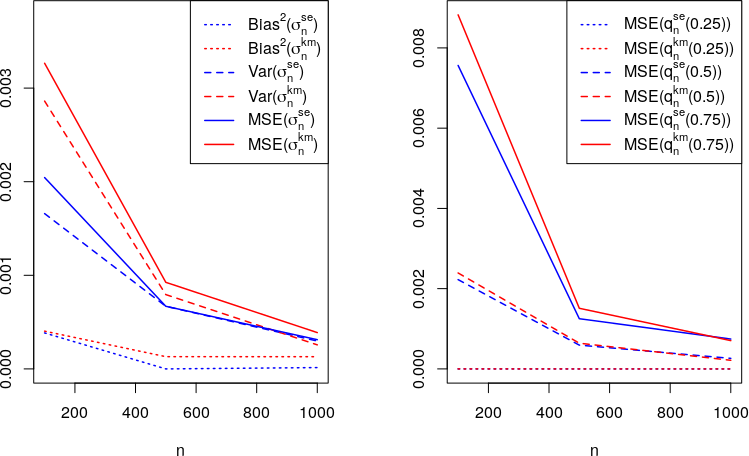
\includegraphics[width=0.9\textwidth]{./figures/weiwei_mse2}
	\end{center}
	\caption{Results for Simulation 2. left: bias, variance and MSE for $\sigma_n^{se}$ and $\sigma_n^{km}$. right: MSE for $q_n^{se}$ and $q_n^{km}$.}
	\label{fig:mse_weiwei}
\end{figure}
%
%
%
\section{Simulation 3} \label{sec:sim_exppar}
Let $X \sim Exp(\alpha)$ and $Y \sim Par(\beta)$. For our model $m$ we obtain in this case
$$m(z,\theta) = \frac{\alpha}{\alpha + \frac{\beta}{z}\I{z \geq \beta}}\mdot$$
For the following simulation we chose $\alpha = 0.5$ and $\beta = 1.2$. The target value was here
$$Var(X) = 4\mdot$$
Figure \ref{fig:dens_exppar} shows the pdf's $f$, $g$ and the censoring model $m$ for this setup.
\clearpage
\begin{figure}[h!]
	\begin{center}
		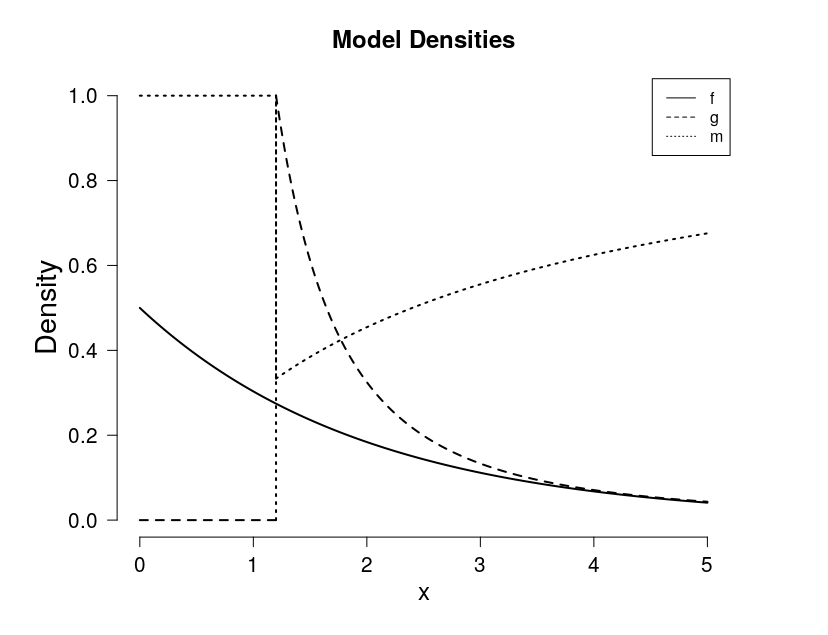
\includegraphics[width=0.8\textwidth]{./figures/exppar_dens}
	\end{center}
	\caption{Probability density functions $f$, $g$ and censoring model $m$ for Simulation 3.}
	\label{fig:dens_exppar}
\end{figure}
%
Note that there are no uncensored observations on $[0,\beta]$. The plot indicates that censoring will especially occur for values in $[1,3]$.
%
The simulation results can be found in tables \ref{tab:res_exppar1} and \ref{tab:res_exppar2}. An illustration of these results is displayed in figure \ref{fig:mse_exppar}.
\begin{table}[h!]
	\begin{center}

%run(n = c(100,500,1000), m = 100, theta = c(0.5, 1.2))
	\begin{tabular}{| l || c | c | c |}	
		\hline
		& $ n = 100 $ & $ n = 500 $ & $ n = 1000 $\\
		\hline
		\hline
%		$Var$ & 4 & 4 & 4\\
%		$U_n^{se}$ & 2.938322 & 3.574439 & 3.726535\\
%		$U_n^km$ & 2.902828 & 3.48581 & 3.681142\\
		$Bias(\sigma_n^{se})$ & -1.061678 & -0.425561 & -0.273465\\
		$Bias(\sigma_n^{km})$ & -1.097172 & -0.51419 & -0.318858\\
		\hline
		$Var(\sigma_n^{se})$ & 2.828115 & 0.852244 & 0.362266\\
		$Var(\sigma_n^{km})$ & 2.991916 & 1.289473 & 0.5611\\
		\hline
		$MSE(\sigma_n^{se})$ & 3.955275 & 1.033346 & 0.437049\\
		$MSE(\sigma_n^{km})$ & 4.195703 & 1.553865 & 0.66277\\
		\hline
		\hline
		$\bar c$ & 0.3029 & 0.30296 & 0.30384\\
		\hline
	\end{tabular}
	\end{center}
	\caption{Results for simulation 3.}
	\label{tab:res_exppar1}
\end{table}\\
The MSE for both, $\sigma_n^{se}$ and $\sigma_n^{km}$, are substantially higher than in the previous examples, especially for $n=100$. However, the MSE decreases substantially as $n$ increases. Again, we can see that the semiparametric approach is performing better than the Kaplan-Meier PLE.
\begin{table}[h!]
	\begin{center}
		
		%run(n = c(100,500,1000), m = 100, theta = c(0.5, 1.2))
		\begin{tabular}{| l || c | c | c |}	
			\hline
			& $ n = 100 $ & $ n = 500 $ & $ n = 1000 $\\
			\hline
			\hline
			$Bias(q^{se}_n(0.25)) $ & -0.946058 & -0.953076 & -0.948244\\
			$Bias(q^{km}_n(0.25)) $ & -0.946058 & -0.953076 & -0.948244\\
			\hline
			$Bias(q^{se}_n(0.5)) $ & -0.761661 & -0.763693 & -0.751274\\
			$Bias(q^{km}_n(0.5))$ & -0.756513 & -0.758938 & -0.748412\\
			\hline
			$Bias(q^{se}_n(0.75))$ & -1.144379 & -1.062969 & -1.04613\\
			$Bias(q^{km}_n(0.75))$ & -1.164122 & -1.088963 & -1.0535\\
			\hline
			\hline
			$MSE(q^{se}_n(0.25))$ & 0.906359 & 0.910549 & 0.900719\\
			$MSE(q^{km}_n(0.25))$ & 0.906359 & 0.910549 & 0.900719\\
			\hline
			$MSE(q^{se}_n(0.5))$ & 0.615678 & 0.590391 & 0.568224\\
			$MSE(q^{km}_n(0.5))$ & 0.610569 & 0.583492 & 0.564373\\
			\hline
			$MSE(q^{se}_n(0.75))$ & 1.400626 & 1.158716 & 1.109287\\
			$MSE(q^{km}_n(0.75))$ & 1.506353 & 1.222739 & 1.130558\\
			\hline
		\end{tabular}
	\end{center}
	\caption{Results for simulation 3.}
	\label{tab:res_exppar2}
\end{table}\\
%
The Quantiles are substantially underestimated by both estimators in this case. Perhaps that is the reason for the much higher MSE scores for $\sigma_n^{se}$ and $\sigma_n^{km}$.
\begin{figure}[h!]
	\begin{center}
		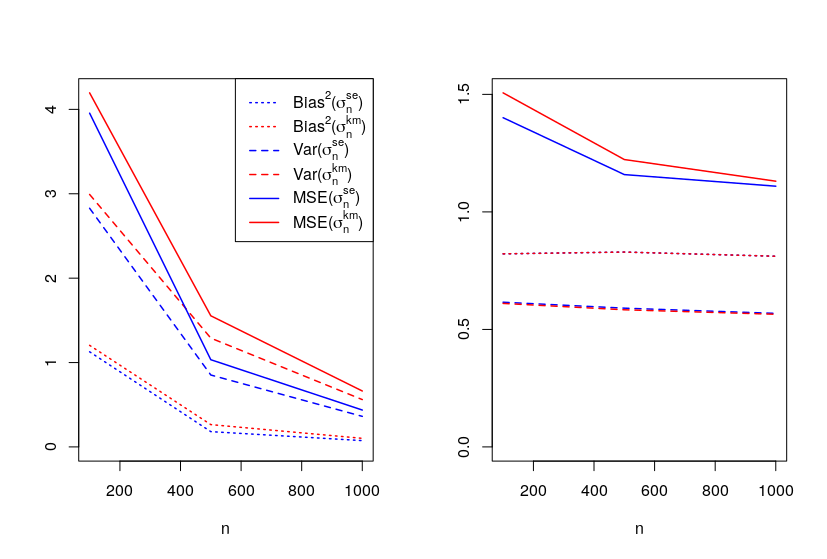
\includegraphics[width=0.9\textwidth]{./figures/exppar_mse2}
	\end{center}
	\caption{Results for Simulation 3. left: bias, variance and MSE for $\sigma_n^{se}$ and $\sigma_n^{km}$. right: MSE for $q_n^{se}$ and $q_n^{km}$.}
	\label{fig:mse_exppar}
\end{figure}